\section{System Architecture}

The proposed controller is organized as a layered architecture that combines a conventional vehicle-level controller with mesoscopic traffic awareness. Figure~\ref{fig:system_architecture} summarizes the four layers: simulation, perception, adaptation, and control.

\begin{figure}[!htbp]
    \centering
    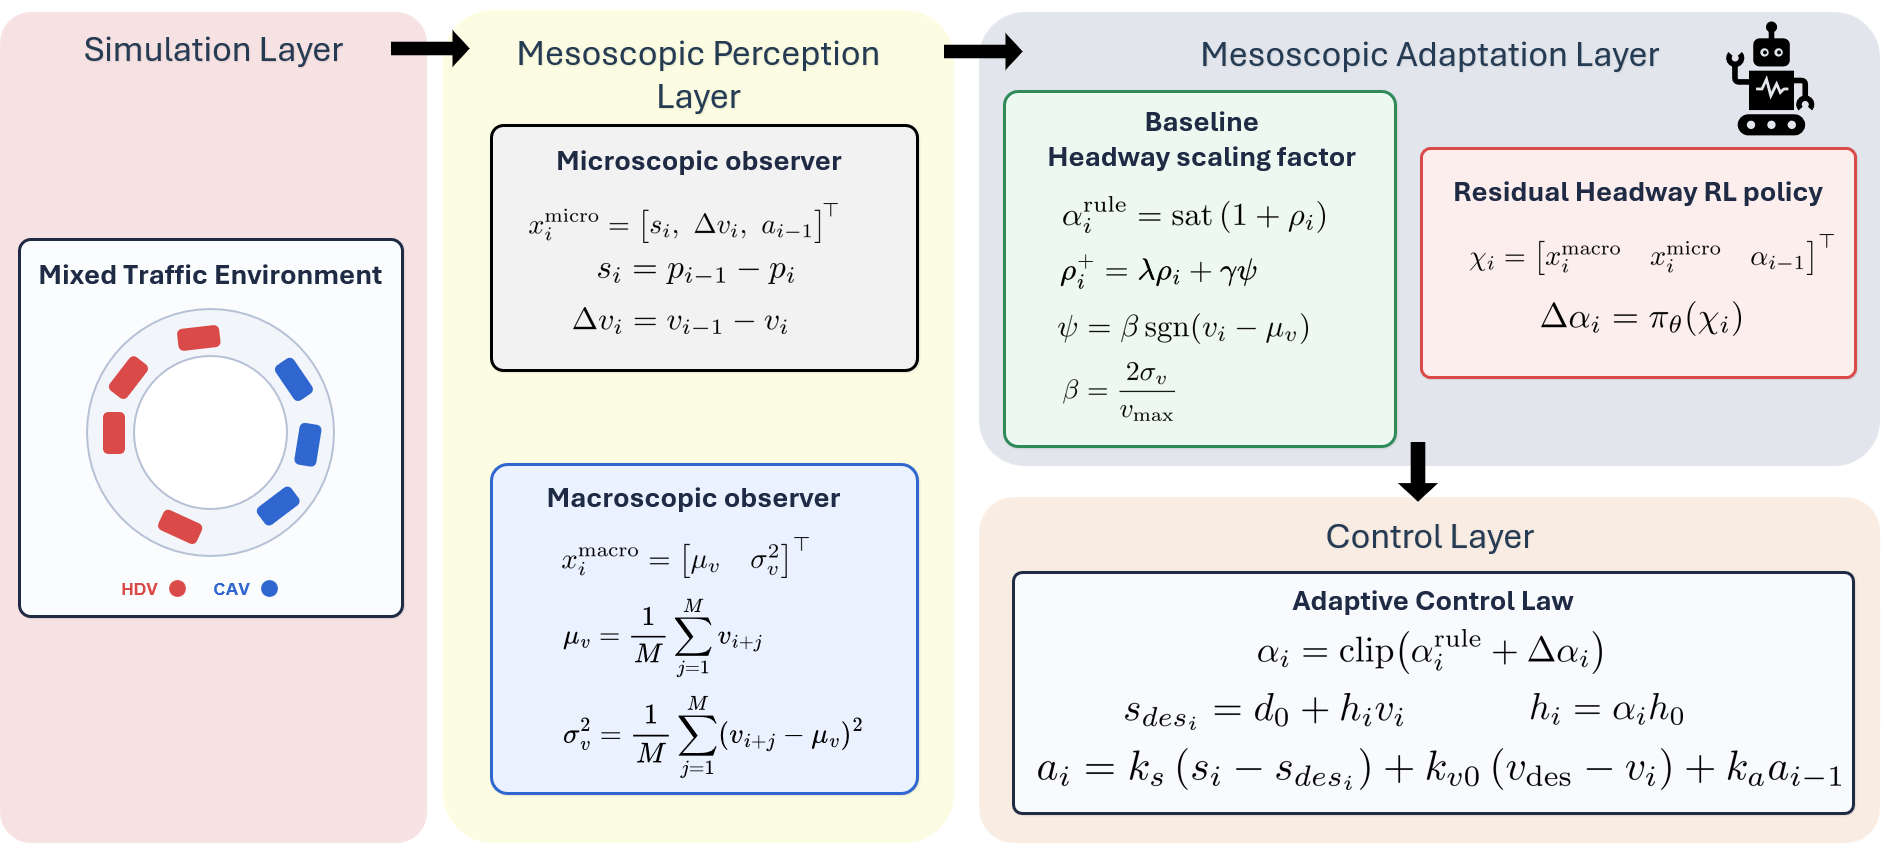
\includegraphics[width=\textwidth]{images/system_architecture.png}
    \caption{Overview of the proposed system architecture.}
    \label{fig:system_architecture}
\end{figure}

\subsection{Overall structure}

At each simulation step, the environment updates all vehicles, the perception layer summarizes the local and upstream traffic state, the adaptation layer converts those observations into a headway adjustment, and the control layer applies the resulting acceleration command. Separating these roles makes the framework easier to debug and makes it explicit what the RL block is allowed to change.

\subsection{Simulation layer}

The simulation layer models a single-lane ring road where HDVs and CAVs coexist. The ring-road setting removes open-boundary entry and exit effects, which makes the appearance of stop-and-go waves easier to observe and compare across methods. This layer provides the positions, velocities, spacing, and leader-acceleration signals used by the upper layers.

\subsection{Mesoscopic perception layer}

The perception layer extracts the information used by the controller. It contains two complementary observers.

\paragraph{Microscopic observer.}
The microscopic observer describes the local car-following situation of vehicle $i$. It uses the spacing, relative velocity, and ego speed:
\[
x_i^{\mathrm{micro}} =
\begin{bmatrix}
s_i & \Delta v_i & a_{i-1}
\end{bmatrix}^{\top},
\]
with
\[
s_i = p_{i-1} - p_i,
\qquad
\Delta v_i = v_{i-1} - v_i.
\]
These variables describe the immediate interaction with the preceding vehicle and are the standard quantities used by longitudinal controllers.

\paragraph{Macroscopic observer.}
The second observer captures collective traffic behavior upstream of the CAV. Instead of looking only at the leader, it summarizes the traffic state over a perception horizon. The two main quantities are the upstream mean velocity and the upstream velocity variance:
\[
x_i^{\mathrm{macro}} =
\begin{bmatrix}
\mu_v & \sigma_v^2
\end{bmatrix}^{\top},
\]
with
\[
\mu_v = \frac{1}{M}\sum_{j=1}^{M} v_{i+j},
\qquad
\sigma_v^2 = \frac{1}{M}\sum_{j=1}^{M}(v_{i+j}-\mu_v)^2.
\]
The mean velocity gives an estimate of the average upstream traffic speed, while the variance indicates how irregular or unstable the traffic stream is.

\subsection{Mesoscopic adaptation layer}

The adaptation layer transforms the observed traffic information into a headway modification for the CAV controller. It contains two parts: a baseline adaptive headway mechanism and a residual reinforcement learning policy.

\paragraph{Baseline adaptive headway.}
The baseline mechanism computes a rule-based headway scaling factor from the macroscopic traffic information. The update can be written as
\[
\alpha_i^{\mathrm{rule}} = \mathrm{sat}(1+\rho_i),
\]
with the internal state
\[
\rho_i^{+} = \lambda \rho_i + \gamma \psi,
\]
and the perception signal
\[
\psi = \beta \,\mathrm{sgn}(v_i-\mu_v),
\qquad
\beta = \frac{2\sigma_v}{v_{\max}}.
\]
This mechanism has a simple interpretation. When upstream traffic becomes more variable, the controller increases the effective headway in order to react more cautiously. When traffic is smoother, the headway can be reduced. The filtering through $\rho_i$ also avoids abrupt parameter changes.

\paragraph{Residual RL policy.}
On top of the baseline adaptation, a residual policy computes a correction term:
\[
\chi_i =
\begin{bmatrix}
    \mu_v & \sigma_v^2 & (v_i-\mu_v) & v_i & s_i & \Delta v_i & a_{i-1} & \alpha_i^{prev}
\end{bmatrix}^{\top},
\qquad
\Delta \alpha_i = \pi_{\theta}(\chi_i).
\]
The role of this block is to refine the rule-based decision without changing the overall structure of the controller. In other words, the adaptive law remains physically interpretable, while the learning block adds flexibility when the traffic situation becomes more complex. The resulting policy input therefore combines mesoscopic information, local car-following variables, and the previously applied headway state in a single 8-dimensional vector.

\subsection{Control layer}

The control layer converts the adapted headway into a longitudinal acceleration command for the CAV. The final scaling factor is
\[
\alpha_i = \mathrm{clip}\!\left(\alpha_i^{\mathrm{rule}} + \Delta \alpha_i\right),
\]
and the corresponding time headway becomes
\[
T_i = \alpha_i T_0.
\]
This adapted headway is then used inside the microscopic CACC/CTH controller:
\[
a_i = k_s\left(s_i - d_0 - T_i v_i\right)
      + k_v \Delta v_i
      + k_a a_{i-1}
      + k_{v0}(v_{\mathrm{des}} - v_i).
\]

The lower-level controller therefore remains a standard feedback law; the upper layers only adapt the time-headway parameter used inside it. This separation preserves a clear physical interpretation of the final command.
